\documentclass[aspectratio=169,11pt]{beamer}

\def\courseTitle{Industrial Security (Master)}
\def\courseSubtitle{Section 04 -- Offensive ICS in Authorised Labs}
\def\sectionNumber{04}
\def\sectionTitle{Offensive ICS in Authorised Labs}

% =====================================================================
% Industrial Security lecture series -- modern Beamer preamble.
%
% Each slide deck must define the following BEFORE \input{}-ing this:
%   \def\courseTitle{...}        e.g. Industrial Security (Bachelor)
%   \def\courseSubtitle{...}     e.g. Section 3 -- Network Architecture
%   \def\sectionNumber{...}      e.g. 03
%   \def\sectionTitle{...}       e.g. Industrial Network Architectures
%
% Optional:
%   \def\courseAuthor{...}       defaults to "Lecture Notes"
%   \def\courseInstitute{...}    defaults to "Department of Computer Science"
%   \def\companyLogo{...}        path to a logo image (PDF/PNG/JPG).
%
% Callout macros (use anywhere inside a frame):
%   \begin{notebox}{title}      ... \end{notebox}
%   \begin{importantbox}{title} ... \end{importantbox}
%   \begin{warningbox}{title}   ... \end{warningbox}
%   \begin{tipbox}{title}       ... \end{tipbox}
%   \begin{defbox}{title}       ... \end{defbox}
%   \begin{takeawaybox}{title}  ... \end{takeawaybox}
%   \begin{quotebox}            ... \end{quotebox}
% =====================================================================

% --- Speaker-notes mode (toggled by Makefile via -usepretex) ----------
% When notesmode=1, build a side-by-side slide+notes PDF for the
% lecturer. When unset/0, build the clean slides-only PDF.
\providecommand{\notesmode}{0}
\ifnum\notesmode=1
  \usepackage{pgfpages}
  \setbeameroption{show notes on second screen=right}
  \setbeamerfont{note page}{size=\small}
\fi

\usepackage[utf8]{inputenc}
\usepackage[T1]{fontenc}
\usepackage[english]{babel}
% Modern type pair: IBM Plex Sans for text, IBM Plex Mono for code.
% Math stays in lmodern; Plex is the dominant family on every text frame.
\usepackage{plex-sans}
\usepackage{plex-mono}
\renewcommand{\familydefault}{\sfdefault}
\usepackage[activate={true,nocompatibility},final,tracking=true,kerning=true,spacing=true,factor=1100,stretch=10,shrink=10]{microtype}
\usepackage{graphicx}
\usepackage{listings}
\usepackage{xcolor}
\usepackage{colortbl}
\usepackage{tikz}
\usepackage{booktabs}
\usepackage{array}
\usepackage{hyperref}
\usepackage{amsmath}
\usepackage{amssymb}
\usepackage{tcolorbox}
\tcbuselibrary{skins, breakable, raster}
\usepackage{fontawesome5}

% =====================================================================
% Shared TikZ styles for the Industrial Security lecture series.
% Loaded by every slide deck and exercise sheet that uses TikZ.
% =====================================================================

\usetikzlibrary{
  arrows.meta,
  shapes,
  shapes.geometric,
  shapes.symbols,
  shapes.multipart,
  positioning,
  fit,
  calc,
  backgrounds,
  decorations.pathmorphing,
  decorations.pathreplacing,
  decorations.text,
  patterns,
  matrix,
  shadows
}

% --- colour palette --------------------------------------------------
\definecolor{isOT}{HTML}{1F4E79}     % OT (deep blue)
\definecolor{isIT}{HTML}{6F2DA8}     % IT (purple)
\definecolor{isSafety}{HTML}{C00000} % safety red
\definecolor{isNet}{HTML}{2E7D32}    % network green
\definecolor{isAttack}{HTML}{B23A48} % attack red
\definecolor{isAccent}{HTML}{E08E0B} % amber
\definecolor{isMute}{HTML}{6B6B6B}   % grey
\definecolor{isLight}{HTML}{EDF2F8}  % light background
\definecolor{isPLC}{HTML}{2C5282}
\definecolor{isHMI}{HTML}{2F855A}
\definecolor{isSCADA}{HTML}{6B46C1}

% --- generic node styles --------------------------------------------
\tikzset{
  isnode/.style={
    draw, rounded corners=2pt, minimum height=8mm, minimum width=18mm,
    font=\small, align=center, thick
  },
  isbox/.style={isnode, fill=isLight},
  plc/.style={isnode, fill=isPLC!15, draw=isPLC, thick},
  hmi/.style={isnode, fill=isHMI!15, draw=isHMI, thick},
  scada/.style={isnode, fill=isSCADA!15, draw=isSCADA, thick},
  sensor/.style={isnode, fill=isNet!10, draw=isNet, minimum height=6mm, minimum width=14mm, font=\scriptsize},
  actuator/.style={isnode, fill=isAccent!15, draw=isAccent, minimum height=6mm, minimum width=14mm, font=\scriptsize},
  firewall/.style={isnode, fill=isAttack!15, draw=isAttack, thick},
  server/.style={isnode, fill=isMute!15, draw=isMute!80, thick},
  switch/.style={isnode, fill=isLight, draw=black!60, minimum height=6mm, minimum width=14mm, font=\scriptsize},
  workstation/.style={isnode, fill=white, draw=isOT, thick},
  attacker/.style={isnode, fill=isAttack!20, draw=isAttack, thick, font=\small\bfseries},
  inetnode/.style={draw, ellipse, minimum width=24mm, minimum height=10mm, font=\scriptsize, fill=isLight, thick},
  process/.style={isnode, fill=isOT!15, draw=isOT, thick, minimum width=24mm},
  zone/.style={
    draw, rounded corners=4pt, thick, dashed, inner sep=4mm
  },
  conduit/.style={-{Stealth[length=2.5mm]}, thick, isNet!80!black},
  attack/.style={-{Stealth[length=2.5mm]}, thick, isAttack, dashed},
  flow/.style={-{Stealth[length=2.5mm]}, thick, isOT!70!black},
  netline/.style={thick, black!60},
  axisline/.style={-{Stealth[length=2mm]}, thick, black!70},
  tag/.style={font=\scriptsize\itshape, fill=white, inner sep=1pt},
  level/.style={
    draw, fill=isLight, minimum width=0.85\linewidth, minimum height=8mm,
    font=\small, anchor=west
  },
  brace/.style={decorate, decoration={brace, amplitude=4pt, raise=2pt}},
  legendbox/.style={draw, rounded corners=2pt, fill=isLight, inner sep=2mm, font=\scriptsize, align=left}
}

% --- handy macros ----------------------------------------------------
% \plcicon, \hmiicon etc as simple labelled boxes; useful inline.
\newcommand{\plcicon}[1][PLC]{\tikz[baseline=-0.6ex]{\node[plc, minimum width=10mm, minimum height=5mm, font=\scriptsize, inner sep=1pt]{#1};}}
\newcommand{\hmiicon}[1][HMI]{\tikz[baseline=-0.6ex]{\node[hmi, minimum width=10mm, minimum height=5mm, font=\scriptsize, inner sep=1pt]{#1};}}
\newcommand{\fwicon}[1][FW]{\tikz[baseline=-0.6ex]{\node[firewall, minimum width=10mm, minimum height=5mm, font=\scriptsize, inner sep=1pt]{#1};}}


\graphicspath{{.}{../../../template/}}

% --- defaults --------------------------------------------------------
\providecommand{\courseAuthor}{Lecture Notes}
\providecommand{\courseInstitute}{Department of Computer Science}
\providecommand{\companyLogo}{logo}

% --- modern palette --------------------------------------------------
\definecolor{slideAccent}{HTML}{1F4E79}       % primary navy
\definecolor{slideSecondary}{HTML}{E08E0B}    % amber accent

% --- Corporate branding overrides ------------------------------------
% A user-editable `branding.tex` at the repo root can override the
% logo path, author/institute lines, and brand colours. If the file is
% missing the built-in defaults above stay in effect.
\IfFileExists{../../../branding.tex}{% =====================================================================
% Corporate / institutional branding -- single file to customise the
% look of the entire course (slides, notes, exercises, labs).
%
% HOW TO REBRAND IN UNDER A MINUTE:
%   1. Replace `branding/logo.pdf` with your own logo
%      (PDF preferred; PNG and JPG also work -- name it `logo.<ext>`).
%   2. (Optional) change the two colours below to your brand palette.
%   3. (Optional) override the author/institute lines below.
%   4. Re-run `make` at the repo root. That's it.
%
% Everything in this file has sensible defaults; you can delete a line
% to fall back to the built-in defaults, or comment it out.
%
% This file is loaded automatically by the slides, exercise, and lab
% preambles -- you never need to \input it manually.
% =====================================================================

% --- Logo --------------------------------------------------------------
% Path is resolved from each leaf-build directory; the default points at
% the shared `branding/` folder at the repo root. If you put your logo
% somewhere else, set the full or relative path here (without extension):
\renewcommand{\companyLogo}{../../../branding/logo}

% --- Author / institute (appears on the title page footer) ------------
\renewcommand{\courseAuthor}{}
\renewcommand{\courseInstitute}{}

% --- Brand colours ----------------------------------------------------
% slideAccent      = primary brand colour (title bands, accent rule)
% slideSecondary   = secondary brand colour (section badge, highlight)
% Both use HTML hex codes. Keep enough contrast against white text.
\definecolor{slideAccent}{HTML}{00205B}      % deep navy
\definecolor{slideSecondary}{HTML}{00A0DC}   % light blue accent
}{}
\definecolor{slideTitle}{HTML}{0F2A44}        % near-black navy
\definecolor{slideMuted}{HTML}{6B6B6B}
\definecolor{slideBg}{HTML}{FFFFFF}
\definecolor{slidePanel}{HTML}{F4F7FB}
\definecolor{slideRule}{HTML}{D6DEE8}

% Callout colours
\definecolor{calNote}{HTML}{1F4E79}
\definecolor{calImportant}{HTML}{B23A48}
\definecolor{calWarning}{HTML}{C77700}
\definecolor{calTip}{HTML}{2E7D32}
\definecolor{calDef}{HTML}{6B46C1}
\definecolor{calTake}{HTML}{0F2A44}

% --- beamer theme ---------------------------------------------------
\useinnertheme{rectangles}
\usefonttheme{professionalfonts}

\setbeamertemplate{navigation symbols}{}
\setbeamertemplate{itemize items}[circle]
\setbeamertemplate{enumerate items}[default]
\setbeamertemplate{section in toc}[ball numbered]
\setbeamercolor{section in toc}{fg=slideTitle}

% Colours
\setbeamercolor{normal text}{fg=slideTitle, bg=slideBg}
\setbeamercolor{title}{fg=slideAccent}
\setbeamercolor{subtitle}{fg=slideMuted}
\setbeamercolor{frametitle}{fg=slideAccent}
\setbeamercolor{structure}{fg=slideAccent}
\setbeamercolor{itemize item}{fg=slideAccent}
\setbeamercolor{itemize subitem}{fg=slideSecondary}
\setbeamercolor{block title}{fg=white, bg=slideAccent}
\setbeamercolor{block body}{fg=slideTitle, bg=slidePanel}
\setbeamercolor{alerted text}{fg=slideSecondary}

% Fonts
\setbeamerfont{title}{series=\bfseries, size=\Large}
\setbeamerfont{subtitle}{series=\mdseries, size=\normalsize}
\setbeamerfont{frametitle}{series=\bfseries, size=\large}
\setbeamerfont{block title}{series=\bfseries, size=\normalsize}
\setbeamerfont{footline}{size=\tiny}

% --- frametitle: title bar + accent underline + section badge -------
% The accent rules are wrapped in a zero-width box so they never
% contribute to the surrounding hbox width (no Overfull warnings).
\setbeamertemplate{frametitle}{%
  \nointerlineskip
  \begin{beamercolorbox}[wd=\paperwidth, ht=2.8ex, dp=1.6ex, leftskip=1.2em, rightskip=1.2em]{frametitle}%
    \usebeamerfont{frametitle}\insertframetitle%
    \hfill
    {\color{slideMuted}\small \sectionNumber}%
  \end{beamercolorbox}%
  \nointerlineskip
  \makebox[0pt][l]{\hspace*{1.2em}\textcolor{slideSecondary}{\rule{2.5em}{1pt}}\textcolor{slideAccent}{\rule{\dimexpr\paperwidth-3.7em\relax}{1pt}}}%
  \par\vskip4pt
}

% --- footer ---------------------------------------------------------
\defbeamertemplate*{footline}{is-footer}{%
  \leavevmode%
  \hbox{%
    \begin{beamercolorbox}[wd=.55\paperwidth, ht=2.4ex, dp=1ex, leftskip=1em]{author in head/foot}%
      {\color{slideMuted}\tiny \courseTitle{} \;\; $\bullet$ \;\; Section \sectionNumber{} -- \sectionTitle}%
    \end{beamercolorbox}%
    \begin{beamercolorbox}[wd=.45\paperwidth, ht=2.4ex, dp=1ex, rightskip=1em]{title in head/foot}%
      \hfill {\color{slideMuted}\tiny \insertframenumber{} / \inserttotalframenumber}%
    \end{beamercolorbox}%
  }%
  \vskip2pt
}

% --- listings -------------------------------------------------------
\definecolor{codebg}{HTML}{F4F7FB}
\definecolor{codekw}{HTML}{0F2A44}
\definecolor{codestr}{HTML}{8B3A3A}
\definecolor{codecom}{HTML}{5A7D54}

\lstset{
    backgroundcolor=\color{codebg},
    basicstyle=\ttfamily\scriptsize\color{slideTitle},
    keywordstyle=\color{codekw}\bfseries,
    stringstyle=\color{codestr},
    commentstyle=\color{codecom}\itshape,
    breaklines=true,
    frame=leftline,
    framerule=2pt,
    rulecolor=\color{slideAccent},
    numbers=left,
    numberstyle=\tiny\color{slideMuted},
    numbersep=8pt,
    showstringspaces=false,
    tabsize=2,
    captionpos=b,
    xleftmargin=0.6em
}

% --- callout boxes --------------------------------------------------
% Shared base style for all callout boxes.
% Subtle drop shadow gives the boxes a hint of elevation without distraction.
\tcbset{
  isCallout/.style={
    enhanced, breakable, sharp corners=northeast,
    arc=2pt, boxrule=0pt,
    leftrule=3pt,
    fonttitle=\bfseries\small,
    coltitle=white,
    fontupper=\small,
    left=2mm, right=2mm, top=1.5mm, bottom=1.5mm,
    drop fuzzy shadow=black!30,
    title={#1}
  }
}

\newtcolorbox{notebox}[1]{
  isCallout={#1},
  colback=calNote!8, colframe=calNote, leftrule=3pt,
  colbacktitle=calNote, attach boxed title to top left={xshift=2mm, yshift=-1.2mm},
  boxed title style={colback=calNote, arc=1pt, boxrule=0pt, left=2mm, right=2mm, top=0.5mm, bottom=0.5mm}
}

\newtcolorbox{importantbox}[1]{
  isCallout={#1},
  colback=calImportant!7, colframe=calImportant, leftrule=4pt,
  colbacktitle=calImportant, attach boxed title to top left={xshift=2mm, yshift=-1.2mm},
  boxed title style={colback=calImportant, arc=1pt, boxrule=0pt, left=2mm, right=2mm, top=0.5mm, bottom=0.5mm}
}

\newtcolorbox{warningbox}[1]{
  isCallout={#1},
  colback=calWarning!10, colframe=calWarning, leftrule=4pt,
  colbacktitle=calWarning, attach boxed title to top left={xshift=2mm, yshift=-1.2mm},
  boxed title style={colback=calWarning, arc=1pt, boxrule=0pt, left=2mm, right=2mm, top=0.5mm, bottom=0.5mm}
}

% Alias warnbox = warningbox, with an optional title (default = "Caution")
\newtcolorbox{warnbox}[1][Caution]{
  isCallout={#1},
  colback=calWarning!10, colframe=calWarning, leftrule=4pt,
  colbacktitle=calWarning, attach boxed title to top left={xshift=2mm, yshift=-1.2mm},
  boxed title style={colback=calWarning, arc=1pt, boxrule=0pt, left=2mm, right=2mm, top=0.5mm, bottom=0.5mm}
}

\newtcolorbox{tipbox}[1]{
  isCallout={#1},
  colback=calTip!8, colframe=calTip, leftrule=3pt,
  colbacktitle=calTip, attach boxed title to top left={xshift=2mm, yshift=-1.2mm},
  boxed title style={colback=calTip, arc=1pt, boxrule=0pt, left=2mm, right=2mm, top=0.5mm, bottom=0.5mm}
}

\newtcolorbox{defbox}[1]{
  isCallout={#1},
  colback=calDef!8, colframe=calDef, leftrule=3pt,
  colbacktitle=calDef, attach boxed title to top left={xshift=2mm, yshift=-1.2mm},
  boxed title style={colback=calDef, arc=1pt, boxrule=0pt, left=2mm, right=2mm, top=0.5mm, bottom=0.5mm}
}

\newtcolorbox{takeawaybox}[1]{
  enhanced, breakable, arc=3pt, boxrule=0pt,
  colback=calTake!7, colframe=calTake,
  toptitle=2mm, bottomtitle=2mm,
  fonttitle=\bfseries\normalsize, coltitle=white,
  colbacktitle=calTake,
  fontupper=\small,
  title={\faStar~Key Takeaway: #1},
  left=3mm, right=3mm, top=2mm, bottom=2mm
}

\newtcolorbox{quotebox}{
  enhanced, breakable, arc=2pt, boxrule=0pt,
  colback=slidePanel, colframe=slideMuted,
  leftrule=3pt, top=2mm, bottom=2mm, left=3mm, right=3mm,
  fontupper=\itshape\small,
}

% Convenience: inline highlight badge
\newcommand{\remembertag}{\tikz[baseline=-0.7ex]\node[fill=calImportant, text=white, font=\scriptsize\bfseries, rounded corners=2pt, inner sep=2pt]{REMEMBER};}
\newcommand{\tldr}{\tikz[baseline=-0.7ex]\node[fill=calTake, text=white, font=\scriptsize\bfseries, rounded corners=2pt, inner sep=2pt]{TL;DR};}

% Source attribution: tiny grey line, anchored bottom-left of the content area
% Usage:  \source{Symantec, \emph{W32.Stuxnet Dossier} v1.4, 2011.}
% Multiple sources:  \source{X.\ Y., 2018; Z, 2020.}
\newcommand{\source}[1]{%
  \par\nointerlineskip\vspace{0.4mm}%
  {\color{slideMuted}\fontsize{5.5}{6.5}\selectfont\textit{Source:} #1\par}%
}

% References slide: aggregate citations + further reading at the end of a section.
% Usage:  \referencesframe{ \item ... \item ... }
% The `frame` environment must be written literally in the deck, so this is a
% macro rather than a wrapper environment (beamer collects the frame body and
% trips over \newenvironment wrappers).
%
% allowframebreakstemplate=\insertcontinuationcount silences the trailing roman
% numeral when content fits on a single page.
\setbeamertemplate{frametitle continuation}[from second]
\newcommand{\referencesframe}[1]{%
  \begin{frame}[allowframebreaks]{References -- Section \sectionNumber}
    \fontsize{7.5}{9}\selectfont
    \setlength{\itemsep}{1pt}
    \begin{itemize}#1\end{itemize}
  \end{frame}%
}

% --- title page -----------------------------------------------------
\title[\courseTitle]{\courseTitle}
\subtitle{\courseSubtitle}
\author{\courseAuthor}
\institute{\courseInstitute}
\date{}

% Logo lookup: try the section directory, then the shared template/.
\newcommand{\showlogo}[1][2cm]{%
  \IfFileExists{\companyLogo.pdf}{\includegraphics[width=#1]{\companyLogo}}{%
    \IfFileExists{\companyLogo.png}{\includegraphics[width=#1]{\companyLogo}}{%
      \IfFileExists{\companyLogo.jpg}{\includegraphics[width=#1]{\companyLogo}}{%
        \IfFileExists{../../../template/\companyLogo.pdf}{\includegraphics[width=#1]{../../../template/\companyLogo}}{%
          \rule{0pt}{0pt}}}}}}

\setbeamertemplate{title page}{%
  \begin{tikzpicture}[remember picture, overlay]
    % accent band (taller to fit wrapped titles)
    \fill[slideAccent] (current page.north west) rectangle ([yshift=-3.4cm]current page.north east);
    \fill[slideSecondary] ([yshift=-3.4cm]current page.north west) rectangle ([yshift=-3.55cm]current page.north east);
    % section badge
    \node[fill=slideSecondary, text=white, font=\bfseries\normalsize, rounded corners=3pt, inner sep=4pt, anchor=north west]
      at ([xshift=1.2cm, yshift=-0.7cm]current page.north west) {Section \sectionNumber};
    % Course title (wraps if long)
    \node[anchor=north west, text=white, font=\bfseries\Large, align=left, text width=11cm]
      at ([xshift=1.2cm, yshift=-1.5cm]current page.north west) {\courseTitle};
    % Subtitle (wraps; smaller, separated)
    \node[anchor=north west, text=white, font=\mdseries\small, align=left, text width=11cm]
      at ([xshift=1.2cm, yshift=-2.7cm]current page.north west) {\courseSubtitle};
    \node[anchor=north east] at ([xshift=-1.2cm, yshift=-1.0cm]current page.north east)
      {\showlogo[2cm]};
    \node[anchor=south west, text=slideMuted, font=\small, align=left, text width=11cm]
      at ([xshift=1.2cm, yshift=1.0cm]current page.south west)
      {\textbf{\sectionTitle}\\[2pt]\textit{\courseAuthor}\\{\scriptsize\courseInstitute}};
  \end{tikzpicture}
}

% --- helper macros --------------------------------------------------
\newcommand{\learningobjectives}[1]{%
  \begin{frame}{Learning Objectives}
    \begin{tipbox}{\faGraduationCap~By the end of this section you will be able to}
      \begin{itemize}\setlength{\itemsep}{2pt}#1\end{itemize}
    \end{tipbox}
  \end{frame}}

\newcommand{\sectionoverviewframe}{%
  \begin{frame}[plain,noframenumbering]
    \titlepage
  \end{frame}
  \begin{frame}{Outline -- Section \sectionNumber}
    \tableofcontents
  \end{frame}}

\AtBeginSection[]{%
  \begin{frame}[plain,noframenumbering]
    \begin{tikzpicture}[remember picture, overlay]
      \fill[slideAccent] (current page.north west) rectangle (current page.south east);
      \fill[slideSecondary] ([yshift=-1pt]current page.center -| current page.west)
                            rectangle ([yshift=1pt]current page.center -| current page.east);
      \node[text=white, font=\scriptsize, anchor=south west]
        at ([xshift=1.2cm, yshift=1.0cm]current page.south west)
        {Section \sectionNumber{} -- \sectionTitle};
      \node[text=slideSecondary, font=\bfseries\Huge, anchor=south]
        at ([yshift=0.4cm]current page.center)
        {\thesection};
      \node[text=white, font=\bfseries\LARGE, align=center, anchor=north, text width=12cm]
        at ([yshift=-0.6cm]current page.center)
        {\insertsection};
    \end{tikzpicture}
  \end{frame}}

\newcommand{\closingframe}{%
  \begin{frame}[plain,noframenumbering]
    \begin{tikzpicture}[remember picture, overlay]
      \fill[slideAccent] (current page.north west) rectangle (current page.south east);
      \node[text=white, font=\bfseries\Huge, anchor=center, align=center, text width=14cm]
        at ([yshift=8mm]current page.center) {End of Section \sectionNumber};
      \fill[slideSecondary] ([xshift=-1.5cm, yshift=-4mm]current page.center)
                            rectangle ([xshift=1.5cm, yshift=-6mm]current page.center);
      \node[text=white, font=\large, anchor=north, align=center, text width=14cm]
        at ([yshift=-1.2cm]current page.center) {\sectionTitle};
      \node[text=slideSecondary, font=\normalsize, anchor=south] at ([yshift=1.2cm]current page.south) {Questions and discussion};
      \node[anchor=south east] at ([xshift=-1cm, yshift=1cm]current page.south east) {\showlogo[1.5cm]};
    \end{tikzpicture}
  \end{frame}}


\begin{document}

\sectionoverviewframe

\learningobjectives{
  \item Distinguish authorised testing, red-team exercises, and unauthorised access -- legally and ethically.
  \item Build a contained lab in which destructive testing is safe.
  \item Apply standard ICS-attack techniques (reconnaissance, protocol abuse, logic injection) with full attribution.
  \item Produce findings that the asset owner can act on without re-doing the work.
}

\section{Ethics and Scope}

\begin{frame}{Authorised vs.\ Unauthorised}
\centering
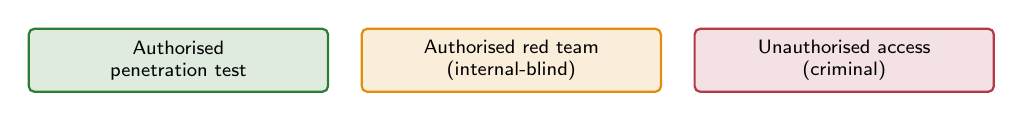
\begin{tikzpicture}[node distance=4mm]
  \node[isbox, fill=isNet!15, draw=isNet, minimum width=38mm, font=\scriptsize, align=center] (auth) {Authorised\\penetration test};
  \node[isbox, fill=isAccent!15, draw=isAccent, minimum width=38mm, font=\scriptsize, align=center, right=of auth] (red) {Authorised red team\\(internal-blind)};
  \node[isbox, fill=isAttack!15, draw=isAttack, minimum width=38mm, font=\scriptsize, align=center, right=of red] (unauth) {Unauthorised access\\(criminal)};
\end{tikzpicture}
\vspace{2mm}
\begin{importantbox}{Paper, not handshake}
``Verbal'' permission is no permission. A signed Rules of Engagement document with named approvers, scope, timing, kill-switch, and reporting path is the gating artefact for any engagement.
\end{importantbox}
\source{NIST SP 800-115 \emph{Technical Guide to Information Security Testing}; PTES Technical Guidelines.}
\end{frame}

\begin{frame}{Legal Surface (EU/DE/US -- partial)}
\begin{itemize}
  \item \textbf{Germany:} \S 202a / 202c StGB criminalise unauthorised access and \emph{preparation tools}; commercial pentesting needs written authorisation.
  \item \textbf{EU CRA (2024/2847):} research safe-harbour for vulnerability disclosure under coordinated terms.
  \item \textbf{US CFAA \& DMCA \S1201:} authorisation contracts grant access; safe-harbour for security research since 2015 rulemaking.
  \item \textbf{ISO/IEC 29147 \& 30111:} normative guidance for coordinated disclosure.
\end{itemize}
\begin{warnbox}
Cross-border engagements need both legal opinions. A US-headquartered firm testing a German plant follows the strictest applicable law.
\end{warnbox}
\source{StGB \S 202a, \S 202c; Directive (EU) 2022/2555; Regulation (EU) 2024/2847; ISO/IEC 29147:2018, 30111:2019.}
\end{frame}

\section{The Lab}

\begin{frame}{Contained Lab Topology}
\centering
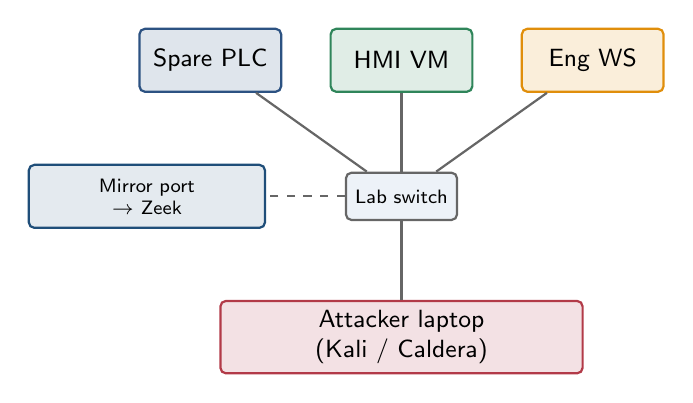
\begin{tikzpicture}[node distance=6mm]
  \node[plc] (plc) {Spare PLC};
  \node[hmi, right=of plc] (hmi) {HMI VM};
  \node[server, right=of hmi, fill=isAccent!15, draw=isAccent] (eng) {Eng WS};
  \node[switch, below=10mm of hmi] (sw) {Lab switch};
  \node[isbox, fill=isAttack!15, draw=isAttack, below=10mm of sw, minimum width=46mm, font=\small, align=center] (att) {Attacker laptop\\(Kali / Caldera)};
  \node[isbox, fill=isOT!12, draw=isOT, left=10mm of sw, minimum width=30mm, font=\scriptsize, align=center] (cap) {Mirror port\\$\to$ Zeek};
  \foreach \n in {plc,hmi,eng}{\draw[netline] (\n) -- (sw);}
  \draw[netline] (sw) -- (att);
  \draw[netline, dashed] (sw) -- (cap);
\end{tikzpicture}
\vspace{2mm}
\begin{tipbox}{Air-gapped, recorded}
No Internet, no host bridge, full PCAP. Every action you take is later auditable to a wall-clock minute.
\end{tipbox}
\end{frame}

\begin{frame}{Lab Equipment Choices}
\centering
\renewcommand{\arraystretch}{1.3}
\footnotesize
\setlength{\tabcolsep}{3pt}
\begin{tabular}{|p{3.0cm}|p{4.8cm}|p{4.4cm}|}
\hline
\rowcolor{slidePanel}
\textbf{Tier} & \textbf{Examples} & \textbf{Best for} \\
\hline
Pure software & OpenPLC, ScadaBR, open62541   & teaching, basic protocol work \\
Mixed         & Spare Siemens S7-1200, Modicon M580 & realistic on-the-wire behaviour \\
Production-grade & Vendor demo kits, donated equipment & vendor-specific exploit research \\
\hline
\end{tabular}
\vspace{2mm}
\begin{notebox}{Donations}
Many vendors donate retired equipment to academic and CERT labs in exchange for confidentiality on findings. Always worth asking.
\end{notebox}
\end{frame}

\section{Tactics}

\begin{frame}{Reconnaissance in OT (passive first)}
\begin{itemize}
  \item ARP / LLDP / CDP listening to enumerate devices.
  \item Passive Zeek capture for 24h to build a baseline.
  \item Vendor banners on web UIs (read-only HTTP GET / robots.txt).
  \item Project files on file shares (engineering WS, contractor laptops).
\end{itemize}
\begin{warnbox}{Active scans on the bench}
Nmap with \texttt{--max-rate} and only NSE scripts known safe for the target. Run once, capture, then decide if a deeper probe is worth the risk.
\end{warnbox}
\source{ICS-CERT (CISA) recommended practices; Dragos \emph{ICS Knowledge Pack}.}
\end{frame}

\begin{frame}{Protocol Abuse Patterns}
\centering
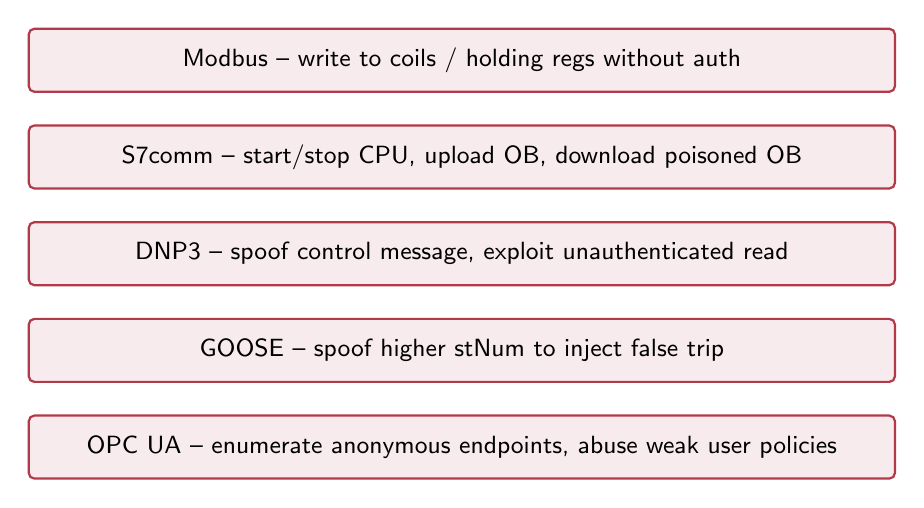
\begin{tikzpicture}[node distance=4mm]
  \node[isbox, fill=isAttack!10, draw=isAttack, minimum width=110mm, font=\small] (a) {Modbus -- write to coils / holding regs without auth};
  \node[isbox, fill=isAttack!10, draw=isAttack, minimum width=110mm, font=\small, below=of a] (b) {S7comm -- start/stop CPU, upload OB, download poisoned OB};
  \node[isbox, fill=isAttack!10, draw=isAttack, minimum width=110mm, font=\small, below=of b] (c) {DNP3 -- spoof control message, exploit unauthenticated read};
  \node[isbox, fill=isAttack!10, draw=isAttack, minimum width=110mm, font=\small, below=of c] (d) {GOOSE -- spoof higher stNum to inject false trip};
  \node[isbox, fill=isAttack!10, draw=isAttack, minimum width=110mm, font=\small, below=of d] (e) {OPC UA -- enumerate anonymous endpoints, abuse weak user policies};
\end{tikzpicture}
\source{MITRE ATT\&CK for ICS, T0855/T0867/T0846/T0848/T0858.}
\end{frame}

\begin{frame}{Logic Injection Workflow}
\centering
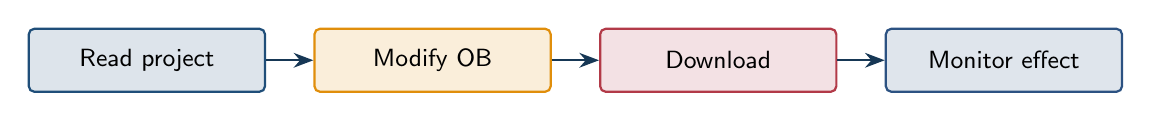
\begin{tikzpicture}[node distance=6mm]
  \node[isbox, fill=isOT!15, draw=isOT, minimum width=30mm, font=\small] (read) {Read project};
  \node[isbox, fill=isAccent!15, draw=isAccent, right=of read, minimum width=30mm, font=\small] (mod) {Modify OB};
  \node[isbox, fill=isAttack!15, draw=isAttack, right=of mod, minimum width=30mm, font=\small] (down) {Download};
  \node[isbox, fill=isPLC!15, draw=isPLC, right=of down, minimum width=30mm, font=\small] (mon) {Monitor effect};
  \foreach \s/\e in {read/mod, mod/down, down/mon}{\draw[flow] (\s) -- (\e);}
\end{tikzpicture}
\vspace{2mm}
\begin{importantbox}{Reversibility}
Always take a verified backup of the original program first, and test the rollback before injecting. ``Oops'' on production hardware is career-ending.
\end{importantbox}
\source{Lab pattern adapted from Klick, J., Lau, S. et al., ``Internet-facing PLCs as a Network Backdoor'', BlackHat USA, 2015.}
\end{frame}

\begin{frame}{Tooling Survey}
\centering
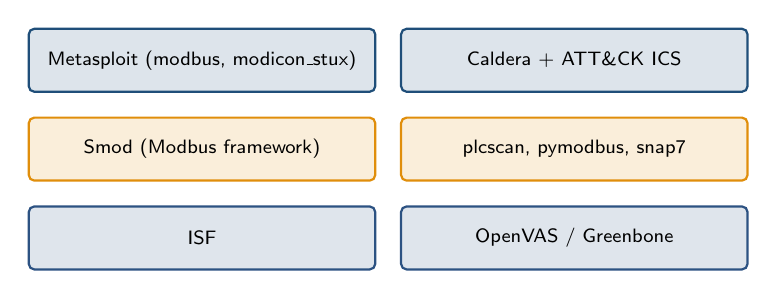
\begin{tikzpicture}[node distance=3mm]
  \node[isbox, fill=isOT!15, draw=isOT, minimum width=44mm, font=\scriptsize] (a) {Metasploit (modbus, modicon\_stux)};
  \node[isbox, fill=isOT!15, draw=isOT, right=of a, minimum width=44mm, font=\scriptsize] (b) {Caldera + ATT\&CK ICS};
  \node[isbox, fill=isAccent!15, draw=isAccent, below=of a, minimum width=44mm, font=\scriptsize] (c) {Smod (Modbus framework)};
  \node[isbox, fill=isAccent!15, draw=isAccent, right=of c, minimum width=44mm, font=\scriptsize] (d) {plcscan, pymodbus, snap7};
  \node[isbox, fill=isPLC!15, draw=isPLC, below=of c, minimum width=44mm, font=\scriptsize] (e) {ISF};
  \node[isbox, fill=isPLC!15, draw=isPLC, right=of e, minimum width=44mm, font=\scriptsize] (f) {OpenVAS / Greenbone};
\end{tikzpicture}
\source{Tool repos: Rapid7 Metasploit; MITRE Caldera; \texttt{theralfbrown/smod}; \texttt{dark-lbp/isf}; Greenbone Networks.}
\end{frame}

\section{Reporting}

\begin{frame}{Report Structure}
\centering
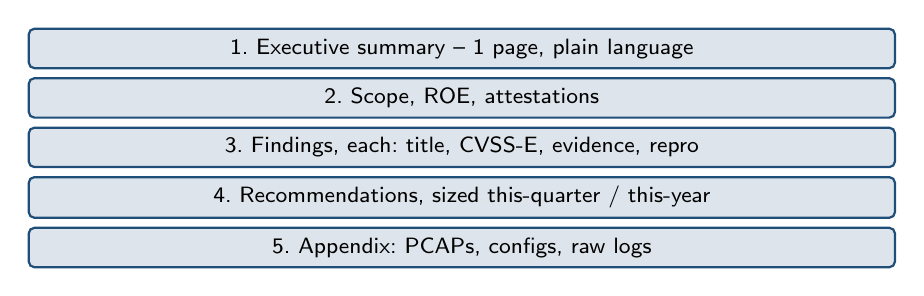
\begin{tikzpicture}[node distance=1mm]
  \node[isbox, fill=isOT!15, draw=isOT, minimum width=110mm, font=\footnotesize, minimum height=5mm] (a) {1.\ Executive summary -- 1 page, plain language};
  \node[isbox, fill=isOT!15, draw=isOT, minimum width=110mm, font=\footnotesize, minimum height=5mm, below=of a] (b) {2.\ Scope, ROE, attestations};
  \node[isbox, fill=isOT!15, draw=isOT, minimum width=110mm, font=\footnotesize, minimum height=5mm, below=of b] (c) {3.\ Findings, each: title, CVSS-E, evidence, repro};
  \node[isbox, fill=isOT!15, draw=isOT, minimum width=110mm, font=\footnotesize, minimum height=5mm, below=of c] (d) {4.\ Recommendations, sized this-quarter / this-year};
  \node[isbox, fill=isOT!15, draw=isOT, minimum width=110mm, font=\footnotesize, minimum height=5mm, below=of d] (e) {5.\ Appendix: PCAPs, configs, raw logs};
\end{tikzpicture}
\vspace{1mm}
\begin{tipbox}{Reproducibility}
A finding without a step-by-step repro is theatre. If the asset owner cannot reproduce it after a week, they will not trust the rest of the report.
\end{tipbox}
\end{frame}

\begin{frame}{Common Reporting Pitfalls}
\begin{itemize}
  \item Listing CVEs without saying which versions are actually in the plant.
  \item Confusing ``vulnerable'' with ``exploitable in this environment''.
  \item Recommendations without owners or timelines.
  \item Findings ranked by CVSS only, not by process-impact.
  \item Reusing screenshots between clients (legal disaster).
\end{itemize}
\begin{warnbox}
The asset owner's safety engineers should be able to read the report and say whether the test \emph{could have} caused a process upset. If not, your scope was wrong.
\end{warnbox}
\end{frame}

\begin{frame}{Summary -- Section \sectionNumber}
\begin{takeawaybox}{Offensive ICS, responsibly}
\begin{itemize}\setlength{\itemsep}{2pt}
  \item Signed Rules of Engagement gate every action -- no signature, no test.
  \item Build a contained lab; never fuzz or inject on production.
  \item Standard ICS-attack patterns (recon, protocol abuse, logic injection) cover most engagements.
  \item Report in plain language with reproducible evidence and prioritised recommendations.
  \item Cross-border work follows the strictest applicable law.
\end{itemize}
\end{takeawaybox}
\end{frame}

\referencesframe{
  \item NIST SP 800-115. \emph{Technical Guide to Information Security Testing and Assessment}, 2008.
  \item PTES. \emph{Penetration Testing Execution Standard}, technical guidelines.
  \item ISO/IEC 29147:2018. \emph{Vulnerability disclosure}.
  \item ISO/IEC 30111:2019. \emph{Vulnerability handling processes}.
  \item Klick, J., Lau, S., Marzin, D., Malchow, J.-O., Roth, V. ``Internet-facing PLCs as a Network Backdoor'', BlackHat USA, 2015.
  \item MITRE. \emph{ATT\&CK for ICS}, knowledge base, current.
  \item MITRE. \emph{Caldera} adversary emulation, with ICS plug-in.
  \item Rapid7. Metasploit Framework, modbus and ICS modules.
  \item Bodungen, C.E., Singer, B., Shbeeb, A., Hilt, S., Wilhoit, K. \emph{Hacking Exposed: Industrial Control Systems}, McGraw-Hill, 2016.
  \item Dragos. \emph{ICS Knowledge Pack} and \emph{Year in Review} reports.
  \item OPC Foundation. \emph{OPC UA Security Bulletin} archive.
  \item Forescout Vedere Labs. ICS vulnerability research outputs.
}

\closingframe

\end{document}
